%doc: Aprendre democracia/APRENDRE DEMOCRACIA.doc
\begin{news}
{2} %columnes
{Aprendre Democràcia}
{El grup de 4t d’ESO ha estat treballant, durant tot aquest primer trimestre, en els continguts del programa “Aprenem a votar”}
{ESO}
{18} %pagesof

%\noindent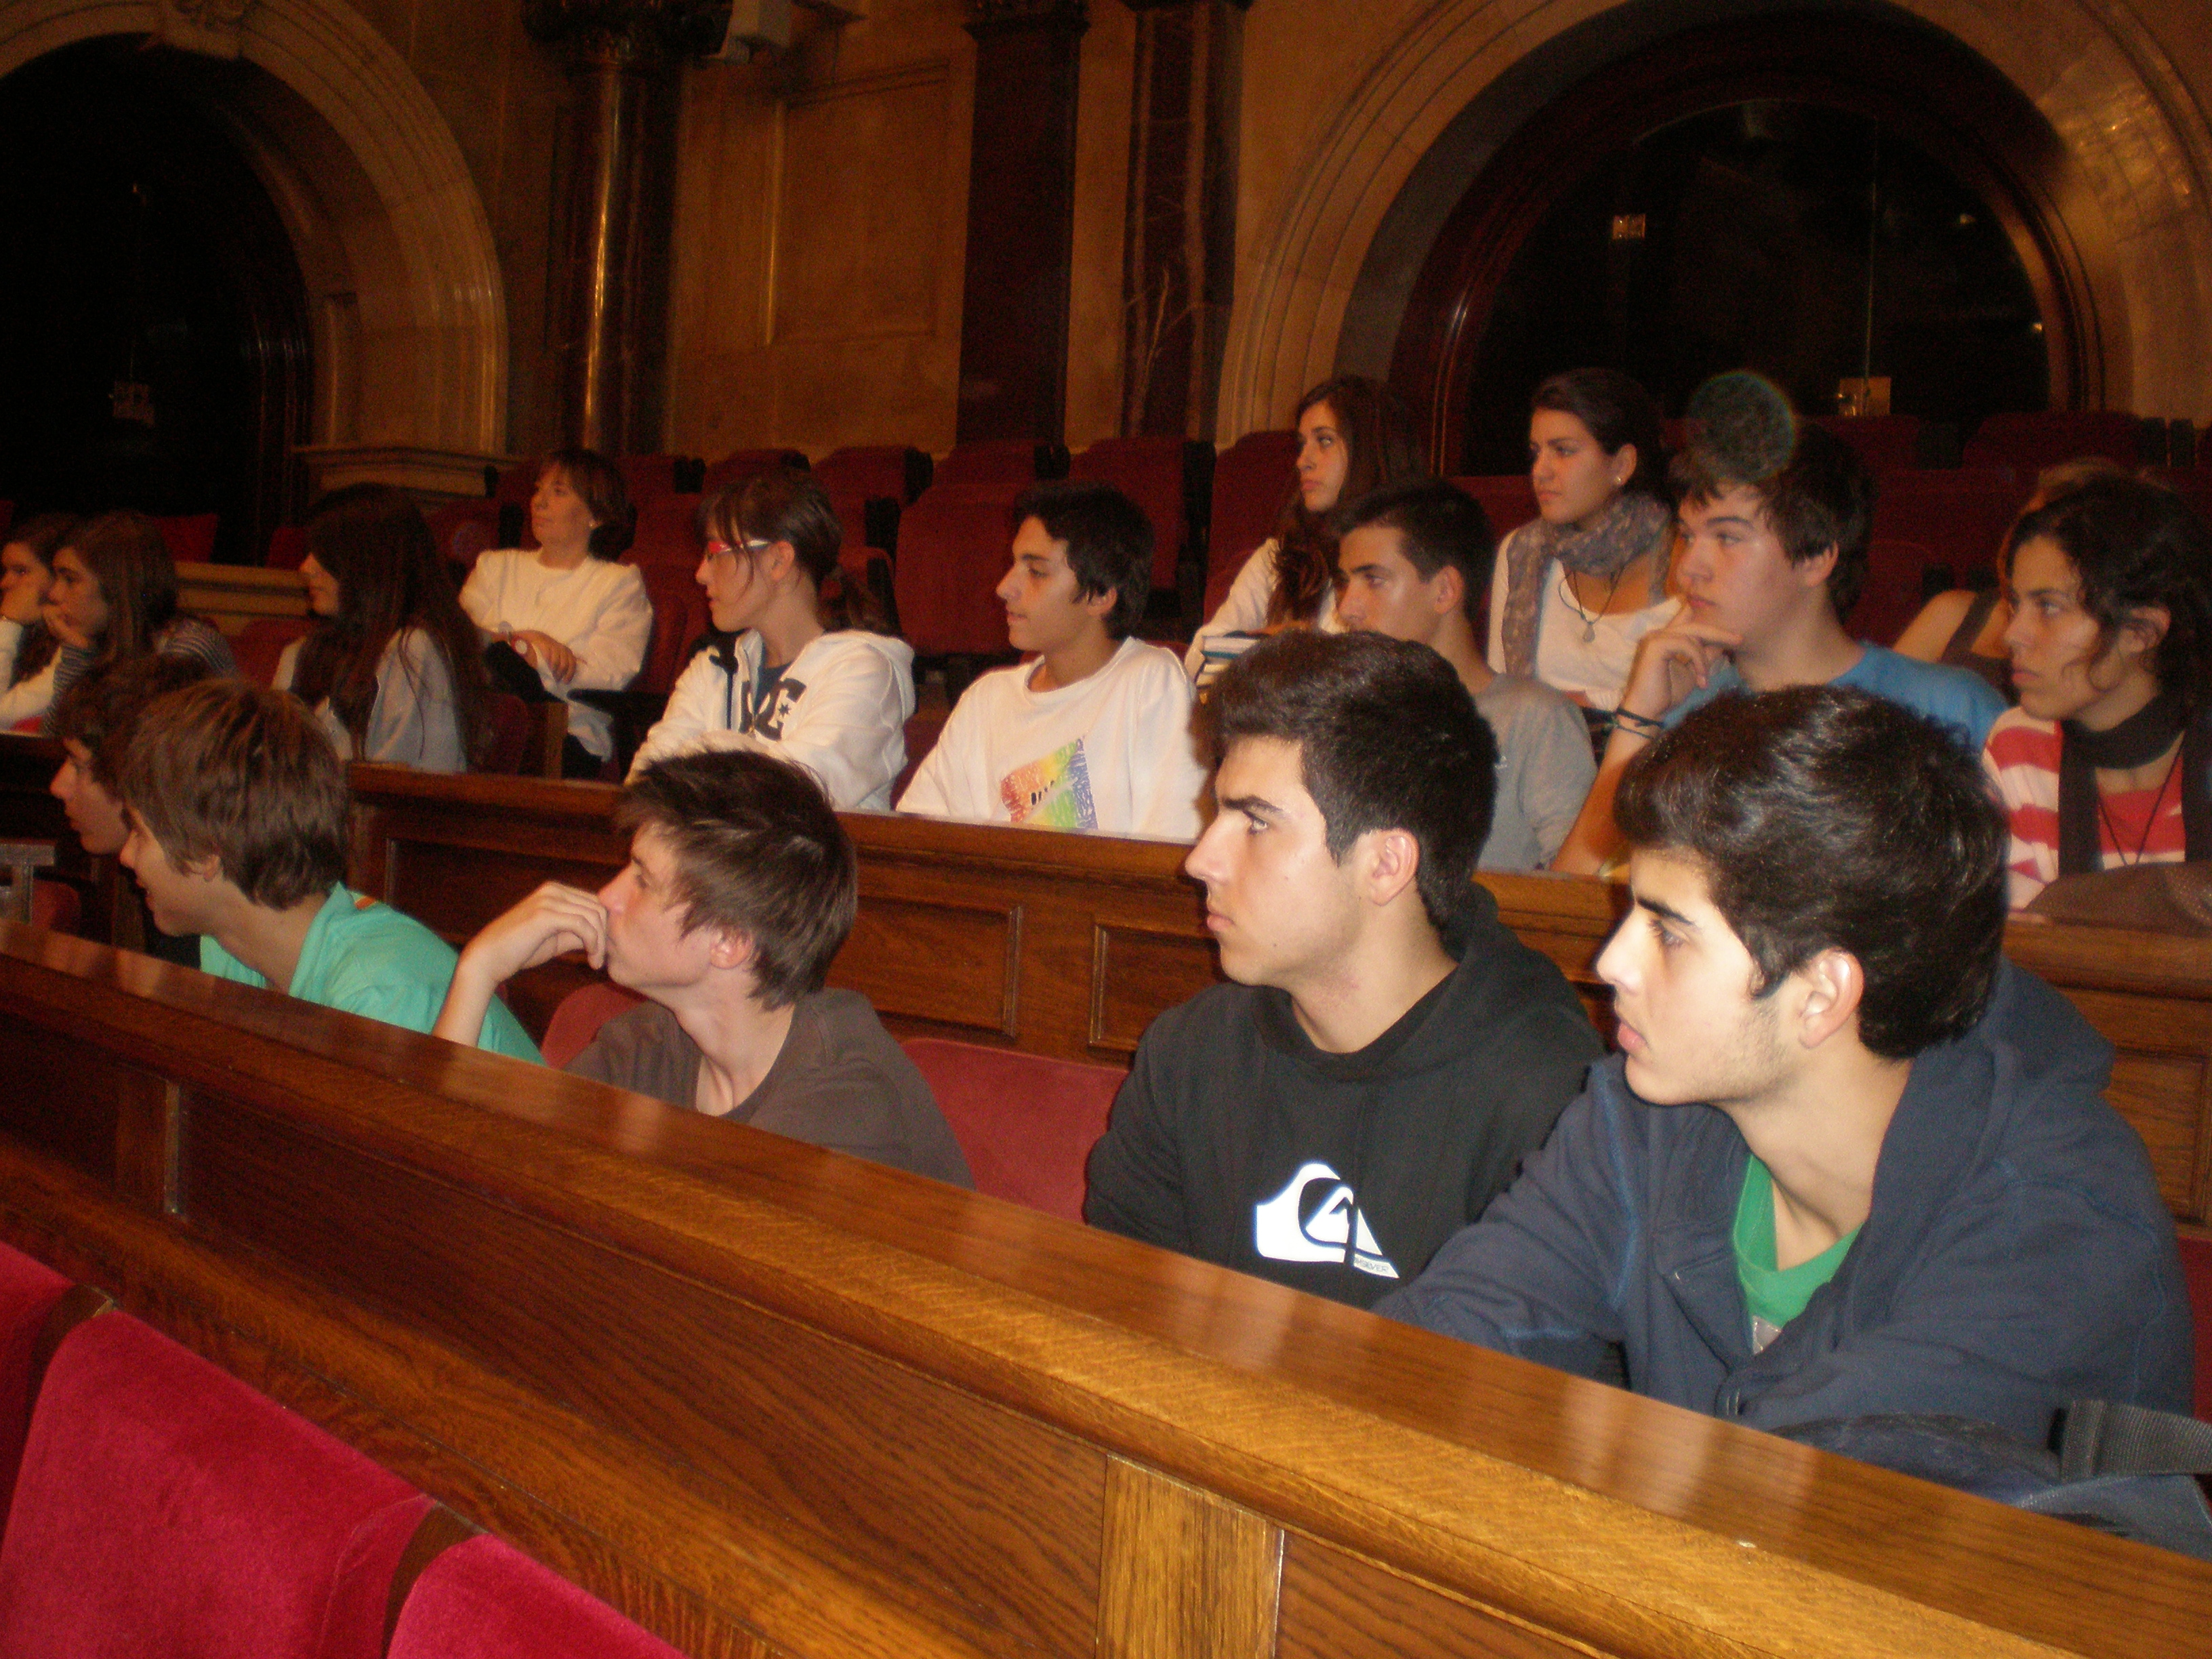
\includegraphics[width=7cm,keepaspectratio]{eso/img/PA220021.JPG}

El nois i noies han anat aprenent que el vot  és una de les diferents maneres d’implicació i de participació política en una democràcia i, tot i que encara no tinguin la majoria d’edat,  van ser convidats a fer una simulació que, de segur, tindrà un impacte important tant en els seus coneixements com en els coneixements que la societat té del que pensa i vol la gent jove.

El nostre centre escolar i el nostre grup de 4t d’ESO han estat escollits per dur a terme aquest procés d’aprenentatge. A través dels exercicis han pogut  conèixer en detall com funcionen les eleccions a Catalunya i com està establert el circuit de representació ciutadana. Els nois i noies, sens dubte,  han fet un exercici de participació molt important per a la vida del nostre país. 

En les fotografies podem veure diferents moments de la visita del grup de 4t de Secundària al Parlament, visita que s’inscrivia dins aquest programa “Aprenem a votar”.

\end{news}

%\noindent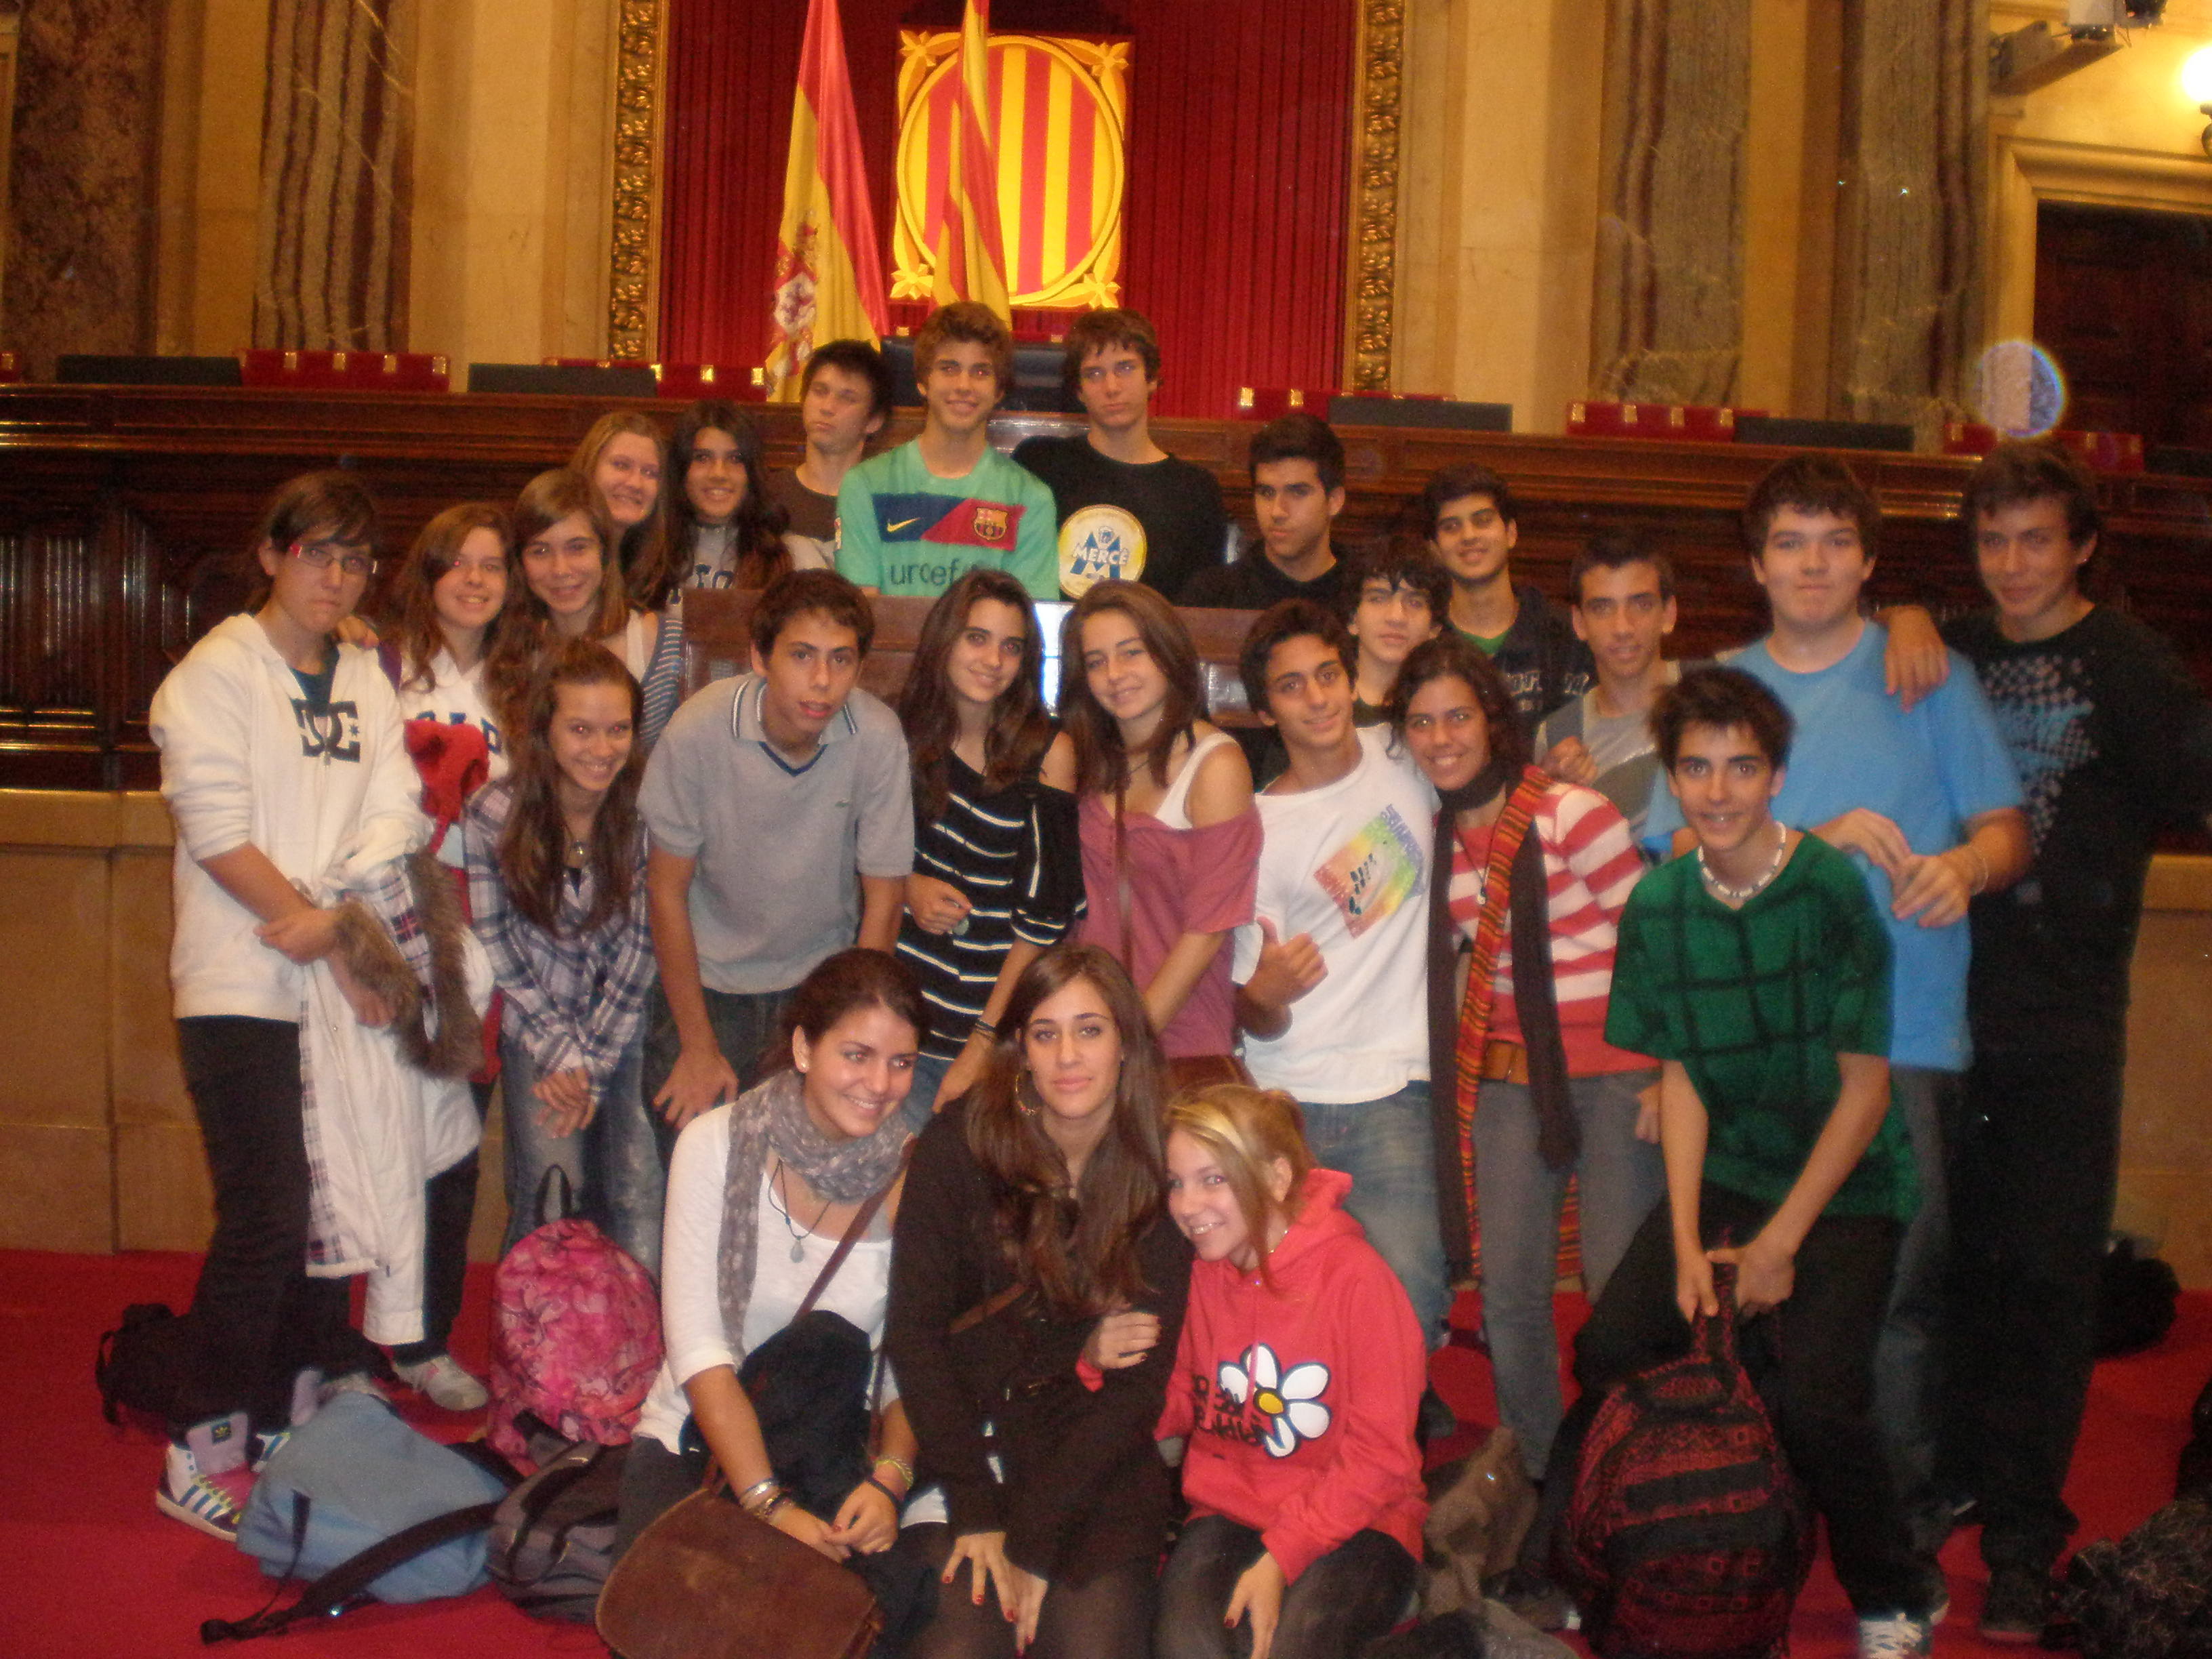
\includegraphics[width=18cm,keepaspectratio]{eso/img/PA220024.JPG}

